\section{Technologievergleich}\label{Technologievergleich}
F\"ur das Projekt soll ein \ac{DMS} verwendet werden, mit welchem sich die vorhandenen Dokumente der \ac{LUBW}, der \ac{GAA} und der \ac{ICT-ENSURE} einfach und bequem in einem System verwalten lassen. Hierbei soll kein \ac{ECM}-Tool von Grund auf neu entwickelt werden. 

Es soll, wie in der Aufgabenstellung im Lastenheft (siehe Kapitel \ref{Lastenheft}) festgehalten, ein passendes Tool gesucht werden, welches die gegebenen Anforderungen bestm\"oglich erf\"ullt. Die Betrachtung erfolgt hierbei unter der Beachtung g\"angiger Standards.

Das \ac{ECM}-Tool, welches f\"ur das Projekt verwendet werden soll, muss die im Folgenden genannten Eigenschaften aufweisen:

\begin{itemize}
 \item Grundlegende Metadatenstandards wie zum Beispiel "`Dublin Core"' und "`EXIF"' m\"ussen unterst\"utzt werden (siehe Kapitel \ref{Analyse Datenbestaende})
 \item Das System muss alle Fachsysteme der \ac{LUBW} vereinen, welche im Kapitel \ref{Stand der Technik} beschrieben sind
 \item Metadaten sollten vom System systematisch gegliedert werden k\"onnen, wie es im Kapitel \ref{Erstellung eines Datenkonzepts} erarbeitet wurde
 \item Das verwendete \ac{ECM}-Tool sollte m\"oglichst viele Schnittstellen bieten, \"uber welche die Daten abgerufen werden k\"onnen
 \item Dateien m\"ussen versioniert werden k\"onnen, um auch \"altere Versionen einsehen zu k\"onnen
 \item Da das Projekt als Prototyp behandelt wird, sollen f\"ur die Umsetzung keine Kosten entstehen
\end{itemize}

Im Folgenden werden nun verschiedene namenhafte \ac{ECM}-Tools vorgestellt und auf die eben genannten Eigenschaften gepr\"uft. Am Ende werden die verschiedenen M\"oglichkeiten verglichen und die beste ausgew\"ahlt.


% Damit ein Tool f\"ur dieses Projekt ausgew\"ahlt werden kann, muss es die im folgenden beschriebenen Eigenschaften beinhalten.

% Das Lastenheft im Kapitel \ref{Lastenheft} besagt, dass im Verlauf der Arbeit ein \ac{ECM}-Tool verwendet werden soll,
\subsection{Agorum Core} \label{Agorum Core}
Bei "`Agorum Core"' handelt es sich um eine Open Source Software, welche von der baden-w\"urttembergischen Firma "`agorum Software"' stammt. "`Agorum Core"' wird in mehreren Varianten angeboten. Zum einem gibt es eine freie Version, welche ohne Lizenzkosten genutzt werden kann, zum anderem gibt es mehrere kostenpflichtige Versionen, die in ihrem Versionsumfang variieren. \cite{agorum_home} 

Agorum bietet viele Funktionen an, welche jedoch in der freien Version nicht vorhanden sind. Um die zus\"atzlichen Funktionen zu nutzen, muss entweder die entsprechende Version, welche die Funktion enth\"alt, gekauft werden oder es muss die entsprechende Funktion hinzugebucht werden.
Somit entstehen auf jeden Fall Kosten, wenn die freie Version von "`Agorum Core"' nicht die gew\"unschten Funktionen bietet. Weiterhin f\"allt negativ auf, dass ein Hinzubuchen von Funktionen unter der freien Version nicht m\"oglich ist. \cite{agorum_preise} \cite{Eval_DMS_Bachelor}

In Abbildung \ref{metadatendesigner agorum}\footnote{\url{http://www.agorum.com/uploads/pics/agorum-core-metadatendesigner_01.png}} ist das Web-Interface von "`agorum core"' zu sehen, wobei hier im Speziellen der "`Metadaten Designer"' zu sehen ist. Dieses Tool ist jedoch ein Zusatzfeature, welches entsprechend hinzugebucht werden muss, was nur innerhalb einer "`Pro"'-Version von "`agorum core"' m\"oglich ist. \cite{agorum_metadesigner_bild}

Der "`Metadaten Designer"' kann verwendet werden, um nutzerspezifische Metadatens\"atze zu erstellen.  Da f\"ur die Arbeit keine "`Pro"'-Version von "`agorum core"' gekauft wurde, kann auf die genaue Verwendung leider nicht eingegangen werden. \cite{agorum_metadaten_designer_video}

\begin{figure}[!ht]
\centering
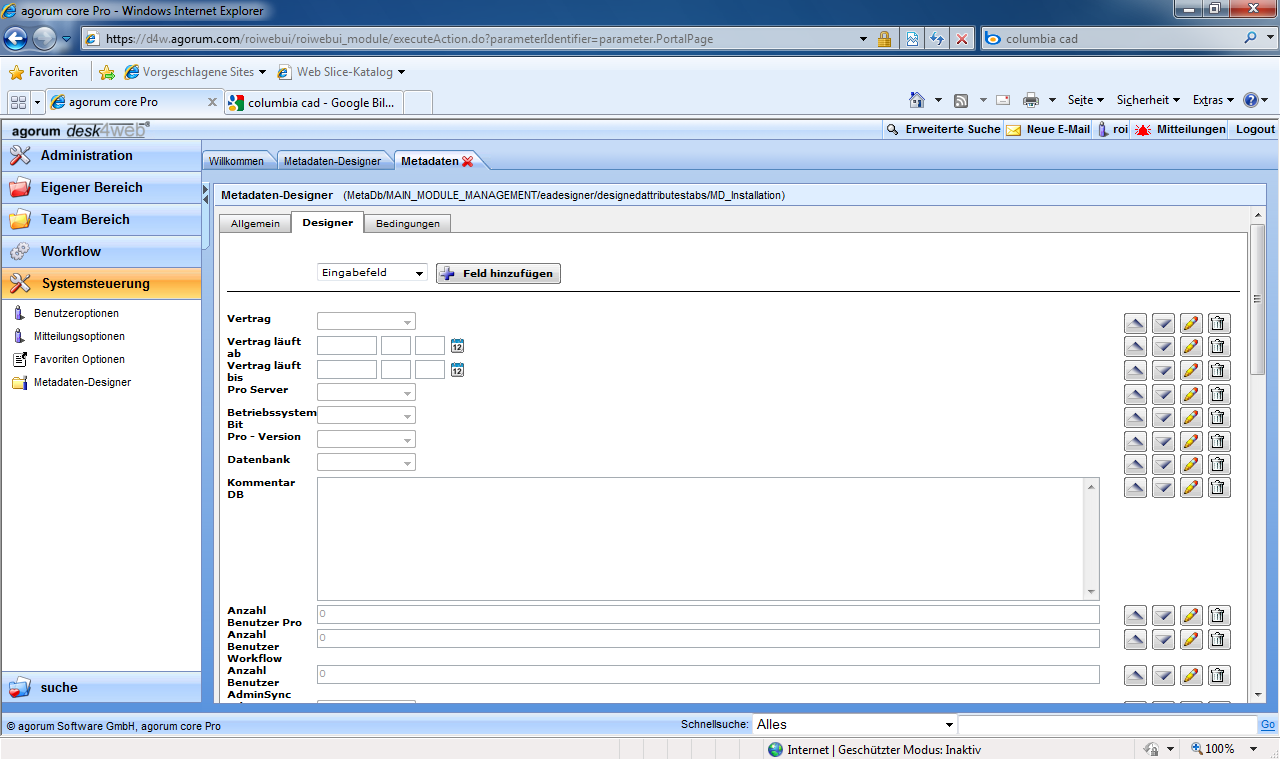
\includegraphics[width=16cm]{Bilder/agorum-core-metadatendesigner.png}
\caption{Metadaten Designer von "`agorum core"' im Web-Interface}
\label{metadatendesigner agorum}
\centering
\end{figure}

Das Einlesen und Bereitstellen von Dokumenten in "`agorum core"' funktioniert schon mit der freien Version. Jedoch kann hier nur eine Standard-Suche und -Ablage verwendet werden. \cite{agorum_preise}

Das automatische Erkennen von Standard-Metadaten in Dateien funktioniert jedoch auch nur mit der entsprechenden "`Pro"'-Version oder einer Zubuchung des Features genau wie die Versionierung von Dateien.

"`agorum core"' verf\"ugt \"uber verschiedene Schnittstellen, welche von Frontends angesprochen werden k\"onnen. 

\subsection{Alfresco} \label{Alfresco}
Alfresco ist eines der heute am weitesten verbreiteten \ac{ECM}-Tools, welches Open Source ist und frei heruntergeladen werden kann.
Flexibilit\"at, Akzeptanz und Skalierbarkeit sind jedoch nur einige der St\"arken, die Alfresco zum Open-Source-Marktf\"uhrer der \ac{ECM}-Branche gemacht haben. \cite{Alfresco_und_Liferay} \cite{Wiki_Alfresco} \cite{Alfresco_Implementation}

Alfresco stammt ebenfalls von einer deutschen Firma, der "`Alfresco Software AG"', und ist somit wie schon agorum auch in der deutschen Sprache verf\"ugbar. Nach angaben der Herstellers, nutzen Namenhafte Unternehmen wie "`Airbus"' oder "`Michelin"' die Software. \cite{Alfresco_Website}

In Abbildung \ref{Alfresco Dashboard} ist das Administrator-Dashboard von Alfresco zu sehen, welches im Webbrowser dargestellt wird.
Im oberen Bildteil ist die Navigationsleiste und das Dash mit m\"oglichen ersten Schritten.

Links ist zum einen das Dash "`Meine Sites"' zu sehen, in welchem alle Seiten zu sehen sind, denen der Nutzer angeh\"ort. Au\ss{}erdem ist darunter ein Dash, welches Aufgaben anzeigt, die vom Benutzer abgearbeitet werden sollen. In Alfresco ist es \"ublich mit Dokumenten und Dateien auch Aufgaben zu verkn\"upfen und Workflows zu gestalten. Dies geht f\"ur jede Datei einzeln oder aber auch f\"ur einen Stack von Dateien.

Im Dash, neben "`Meine Sites"' sind die Aktivit\"aten zu sehen, welche zuletzt passiert sind. Hier kann der Nutzer einstellen, in welchen Zeitraum, f\"ur welche Aktivit\"at oder f\"ur welche Elemente er Aktivit\"aten anzeigen lassen m\"ochte.
Darunter ist ein Dash zu sehen, an welchem ein Nutzer sehen kann, welche Dokumente er zuletzt hochgeladen oder ge\"andert hat.

\begin{figure}[!ht]
\centering
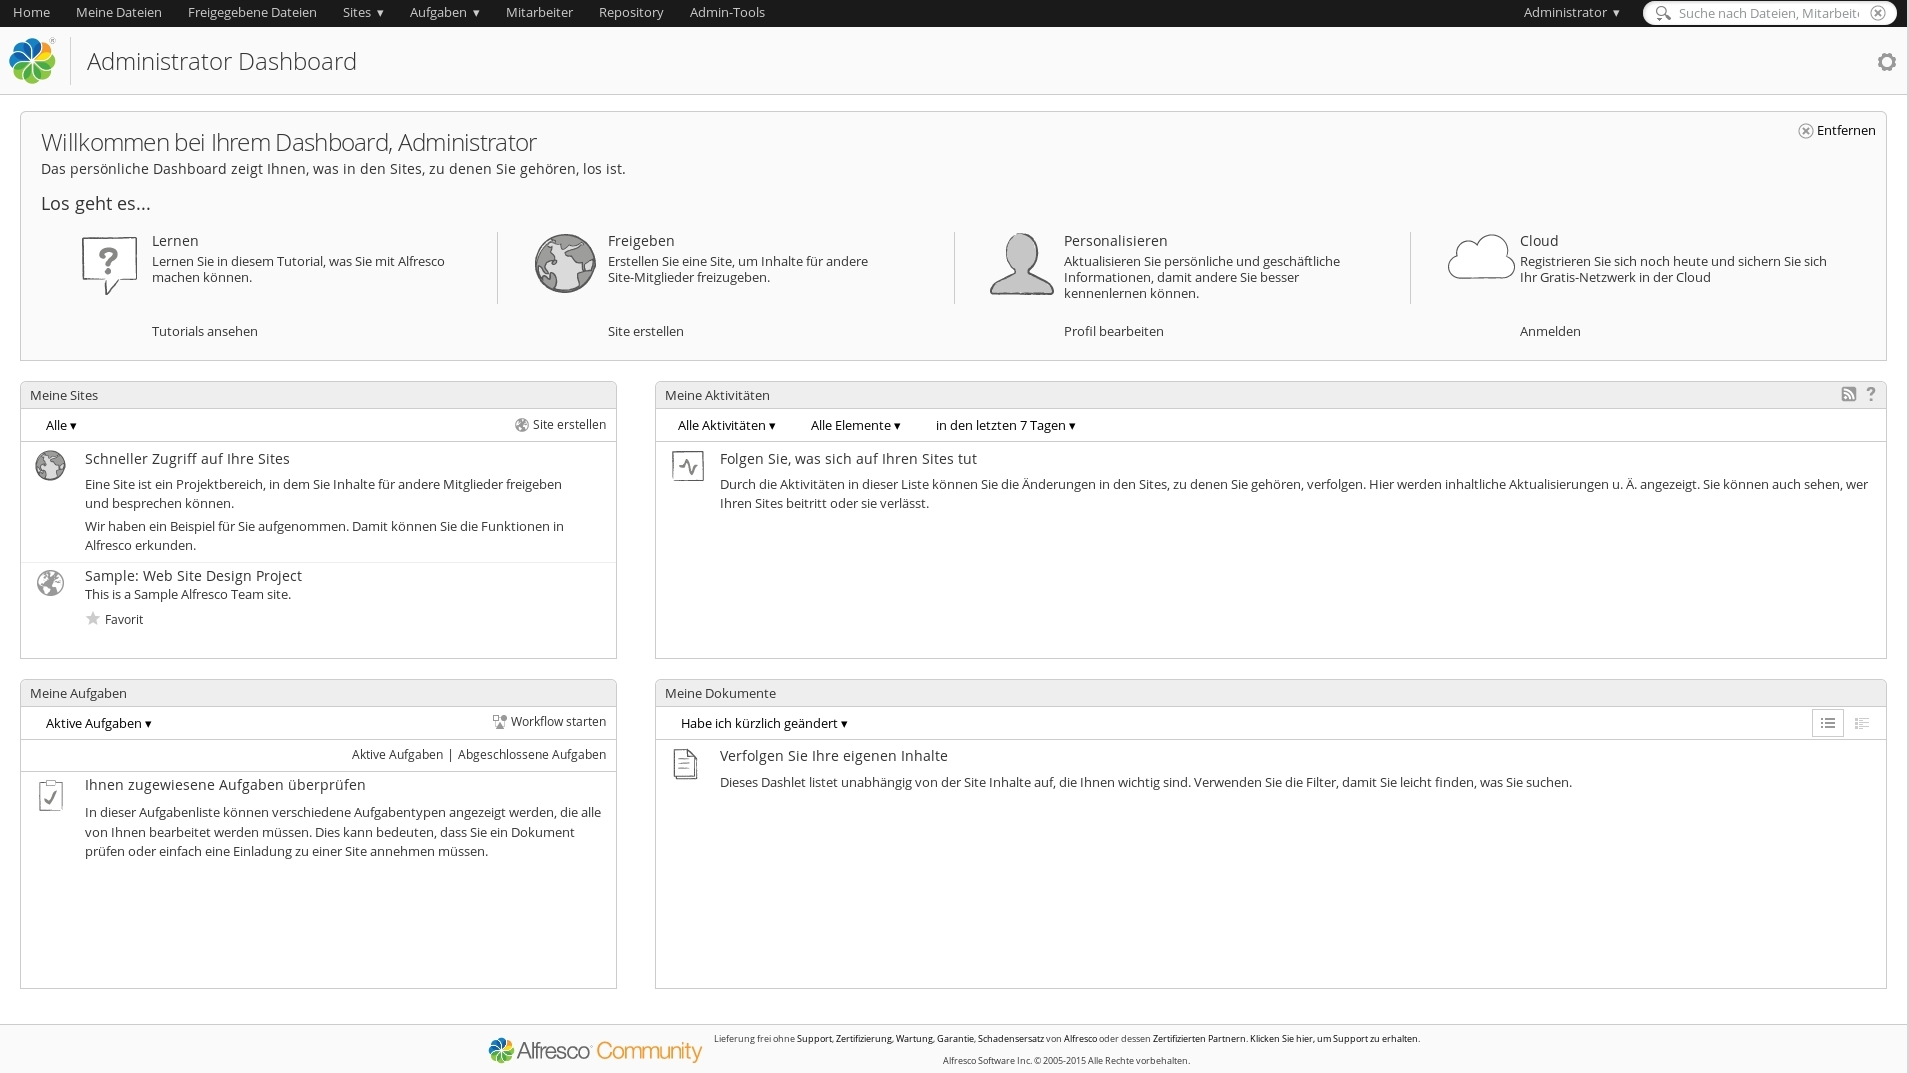
\includegraphics[width=16cm]{Bilder/Alfresco_Oberflaeche.jpg}
\caption{"`Administrator Dashboard"' von Alfresco}
\label{Alfresco Dashboard}
\centering
\end{figure}

Wird eine Datei in Alfresco eingef\"ugt, was per Drag \& Drop geht, werden automatisch schon vorhandene Metadaten aus der Datei herausgelesen. Hierbei werden zum Beispiel bei Bildern auch \ac{Exif}-Daten gelesen und angezeigt, wie in der Abbildung im Anhang \ref{Exif-Metadaten von Alfresco} zu sehen ist. 

Durch die "`Sites"', welche Alfresco bietet, ist es ganz leicht m\"oglich, f\"ur alle bestehenden Systeme der \ac{LUBW} eine eigene "`Site"' zu erstellen. Da Alfresco f\"ur jedes Dokument eine eindeutige ID vergibt, ist es sogar m\"oglich, Dokumente von verschiedenen Seiten zu verlinken.
\cite{Eval_DMS_Bachelor}

Die Vorraussetzung, dass neue Metadaten hinzugef\"ugt werden und diese gruppiert werden k\"onnen, ist in Alfresco gegeben. Dies wird \"uber XML-Definitionen erledigt, welche dann unter Alfresco genutzt und in Workflows eingebaut werden k\"onnen. \cite{Alfresco_Custom_Content_Types} \cite{Professional_Alfresco}

Alfresco bietet die M\"oglichkeit, ein Frontend durch viele verschiedene Schnittstellen anzubinden. Eine Anbindung kann zum Beispiel \"uber \ac{REST}, \"uber WebDAV oder die "`Alfresco One \ac{API}"' erfolgen. \cite{Alfrsco_Doku}

Auch eine Versionierung von Dokumenten ist m\"oglich, wodurch eine neue Version die alte nicht einfach ersetzt. Alte Versionen k\"onnen auch weiterhin eingesehen werden.

Da Alfresco Open Source ist, ist es nicht nur kostenlos (Community Edition), sondern kann auch mit eigenen Tools erweitert werden. Dies kann zum einen \"uber direkte Programmierung im Quellcode geschehen oder zum anderen \"uber Aspekte, da Alfresco aspektorientiert programmiert ist. \cite{Alfresco_und_Liferay}

\subsection{Open-Xchange} \label{Open Xchange}
Open-Xchange, ist ein Groupware-Server, welcher von der Open-Xchange AG, die ihren Sitz in N\"urnberg hat, entwickelt wird und als Open Source unter der \ac{GPL} verf\"ugbar ist. \cite{Xchange_Seite} \cite{Xchange_Golem}

Urspr\"unglich wurde Open-Xchange als E-Mail- und Groupware-L\"osung entwickelt und stellte somit eine alternative zu "`Microsoft Exchange"' dar. \cite{Wiki_Xchange}

In Abbildung \ref{Xchange Dateianzeige} ist die Dateianzeige einer Datei in Open-Xchange dargestellt. Das Bild wurde mit Hilfe der freien Vorschauversion, welche Open-Xchange bietet, erstellt\footnote{\url{http://beta.core.ox.io/welcome/\#pooled\_gold\_source\_en\_eb14204d2e764492ad76045ff7fd4646,trymeWelcome}}. Diese Vorschau ist gut zum Testen der Funktionalit\"at des Servers, befindet sich aber zur Zeit noch in der Beta-Phase. Vorteil durch diese Vorschau ist auf jeden Fall, dass kein Nutzer sich mehr m\"uhsam einen Server zum Testen der Funktionalit\"at aufsetzen muss.

Zu beobachten ist, dass die Oberfl\"ache von Open-Xchange \"ahnlich wie die von Alfresco aussieht, was in Abbildung \ref{Alfresco Dashboard} gut zu erkennen ist. Die liegt zum einen an der \"ahnlichen Gestaltung der Oberfl\"achen, zum anderen daran, dass beide das freie HTML und CSS Framework "`Bootstrap"'\footnote{\url{http://getbootstrap.com/}} verwenden.

Im oberen Teil der Abbildung \ref{Xchange Dateianzeige} ist die Navigationsleiste zu sehen, welche es erm\"oglicht, die gesamte Funktionalit\"at schnell und einfach zu erreichen. Der linke Abschnitt zeigt einen Navigator, der alle Ordner, welche sich gerade im System befinden, darstellt. Mittig ist die Liste der Dateien zu sehen, welche sich im links gew\"ahlten Ordner befinden. W\"ahlt der Nutzer nun eine Datei aus, so erscheint der rechte Bildabschnitt mit einer Dateivorschau und Informationen zur Datei.

Open-Xchange ist leider nicht in der Lage, die schon vorhandenen Metadaten der Datei anzuzeigen, geschweige denn eigene Attribute hinzuzuf\"ugen.

\"Uber viele Schnittstellen ist es m\"oglich, Daten von Open-Xchange auszulesen, so zum Beispiel auch \"uber eine HTTP-\ac{API}. \cite{Oxpedia_HTTP_API}

Leider ist der Schwerpunkt von Open-Xchange eher die Kommunikation \"uber E-Mail und die Verwendung als Groupware. Als \ac{ECM}-Tool, wie es f\"ur die Arbeit ben\"otigt wird, ist es jedoch ungeeignet, da es weder Metadaten einlesen noch verarbeiten kann.

\begin{figure}[!ht]
\centering
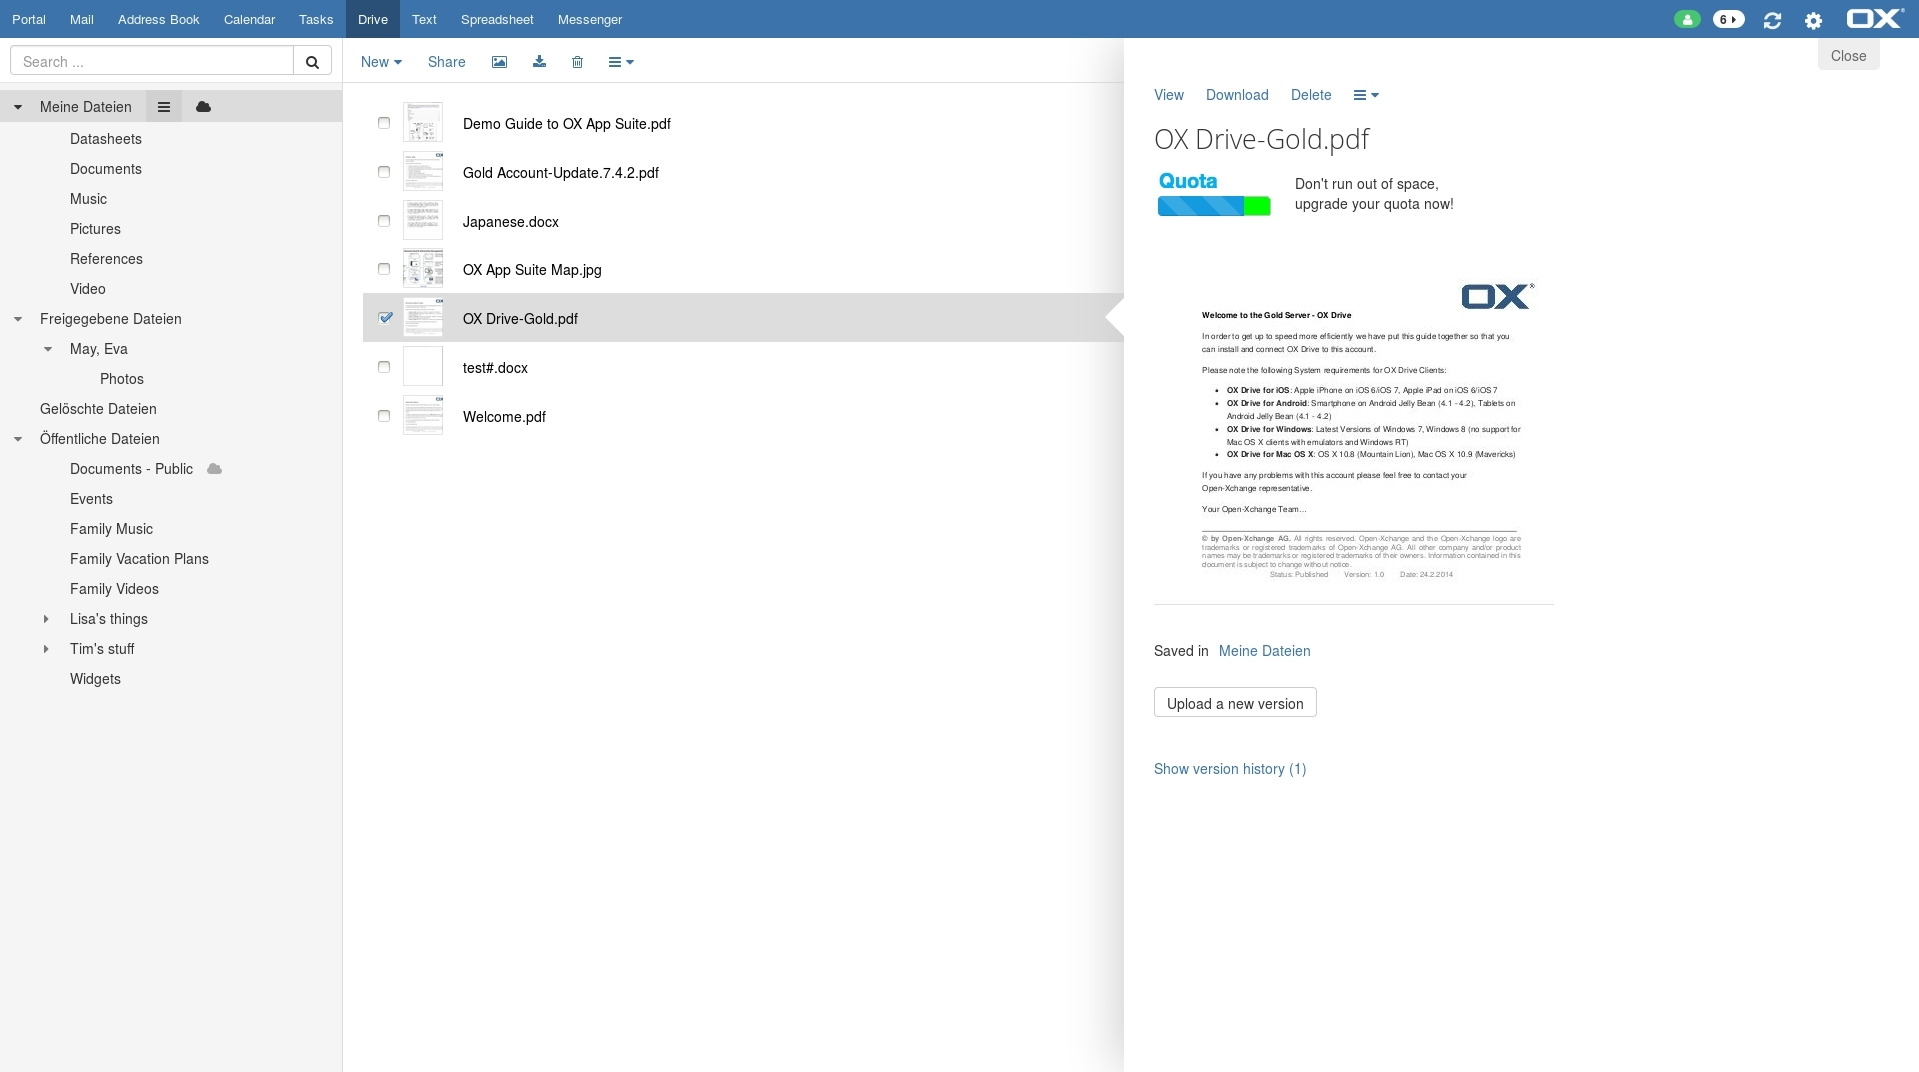
\includegraphics[width=16cm]{Bilder/xchange_Oberflaeche.jpg}
\caption{Datei-Anzeige von Open-Xchange}
\label{Xchange Dateianzeige}
\centering
\end{figure}

\FloatBarrier
\subsection{Liferay als ECM-Tool} \label{Liferay}
F\"ur die Entwicklung des Frontends soll Liferay verwendet werden, welches ein Tool f\"ur die Erstellung von Webportalen ist.
Liferay wird im Kapitel \ref{Implementierung Frontend} genauer beschriebenen.
Da Liferay auch eine Verwaltung f\"ur Dokumente besitzt, wird hier nat\"urlich auch gepr\"uft, ob eine Umsetztung des Projekts nur mit Liferay m\"oglich ist.

Liferay ist eigentlich als Portalserver ausgelegt, bietet jedoch die M\"oglichkeit, Dokumente, die auf einer Webseite ben\"otigt werden, zu speichern und zu verwalten. Hierbei werden beim Hochladen von Dateien die standardisierten Metadaten ausgelesen und angezeigt, bei einem JPEG-Bild w\"aren das zum Beispiel die vorhandenen \ac{Exif}-Daten.

F\"ur die gespeicherten Dateien bietet Liferay eine Versionierung innerhalb des Systems, \"altere Versionen einer Datei k\"onnen jedoch nicht von au\ss{}en aufgerufen werden. Liferay verwendet auch keine IDs, um ein Dokument eindeutig zu identifizieren, verlangt aber eindeutige Namen bei der Speicherung von Dateien, wodurch IDs entfallen. Zur internen Datenbankspeicherung werden nat\"urlich auch IDs verwendet, diese sind jedoch auf der Oberfl\"ache nicht sichtbar und somit nicht nutzbar.

Es k\"onnen im System zus\"atzlich zu den vorhandenen Metadaten eigene Metadatens\"atze erstellt werden, dies geschieht entweder per \ac{UI} oder per XML-Definition.
Leider erm\"oglicht es  Liferay nicht, einen Metadatensatz innerhalb eines Metadatensatzes zu verwenden, wodurch die Strukurierung des Modells verloren gehen w\"urde.

Vorteilig an Liferay ist, dass spezielle Dokumenten-Typen erstellt werden k\"onnen, die alle Metadaten-Schl\"ussel enthalten. So kann zum Beispiel ein Datentyp \ac{FADO}-Urteil speziell f\"ur Urteile aus \ac{FADO} erstellt werden. Leider ist es nicht m\"oglich, einen Metadatensatz zweimal in einen Dokument zu verwenden, wie es bei der Datensammlung \texttt{Urteil} n\"otig w\"are, da sie die Attribute \texttt{Vorgericht} und \texttt{Nachgericht} enth\"alt, welche beide auf ein \texttt{Gericht} verweisen.

Liferay bietet verschiedene Schnittstellen, um nach au\ss{}en hin zu kommunizieren, so zum Beispiel WebDAV.

\subsection{Auswertung der M\"oglichkeiten}\label{Auswertung ECM}
Nach dem in den Abschnitten \ref{Agorum Core}, \ref{Alfresco} und \ref{Open Xchange} die drei wichtigsten Vertreter der \ac{ECM}/\ac{DMS}-Tools
betrachtet wurden, muss nun eine Entscheidung getroffen werden, welches System sich am besten f\"ur das Projekt eignet. Zus\"atzlich wurde im Abschnitt \ref{Liferay} gepr\"uft, ob Liferay als ECM-Tool geeignet ist.

Hierf\"ur wurden die im Abschnitt \ref{Technologievergleich} aufgef\"uhrten Anforderungen noch einmal in Tabellenform dargestellt (siehe Tabelle \ref{Systemvergleich}). Die einzelnen Systeme wurde in der Tabelle nebeneinander gestellt, wobei ein \textcolor{green}{\checkmark} f\"ur volle Umsetzung im System, ein \textcolor{orange}{\checkmark X} f\"ur eine Umsetzung im System gegen Geb\"uhren und ein \textcolor{red}{X} f\"ur keine Umsetzung im System steht.

In der Tabelle \ref{Systemvergleich} f\"allt auf, das "`agorum core"' zwar f\"ur das Projekt geeignet w\"are, jedoch durch die hohen Lizenzkosten nicht verwendet werden kann, wie es im Abschnitt \ref{Agorum Core} schon dargelegt wurde. Die f\"ur die Arbeit ben\"otigten Komponenten sind kostenpflichtig und nur in Verbindung mit einer lizensierten "`Pro"'-Version nutzbar.

Open-Xchange ist eine interessante Alternative f\"ur das von Microsoft stammende Exchange, und ist kostenfrei, da es sich um Open-Source-Software handelt. Jedoch bietet Open-Xchange nicht die Unterst\"utzung, welche f\"ur diese Arbeit ben\"otigt wird. Vor allem in den beiden Punkten, wo es um die Gliederung von Metadaten und die Implementierung von Metadatenstandards geht, kann Open-Xchange nicht mithalten. Da diese Punkte eine sehr hohe Priorisierung haben, kann Open-Xchange nicht verwendet werden.

Das Verwalten, Versionieren und das Anzeigen von Dokumenten funktioniert sehr gut, jedoch wird von Seiten Open-Xchanges aus keine Unterst\"utzung von Metadaten geboten. Eine eigene Implementierung dieser Funktionalit\"at w\"are zwar denkbar, da der Quellcode unter der \ac{GPL} steht, jedoch im Rahmen des zeitlichen Umfangs der Arbeit nicht umsetzbar.

Die vielversprechenste Alternative ist Alfresco, welches alle Anforderungen erf\"ullt. Zum einen ist es Open Source und somit frei verf\"ugbar, zum anderen bietet es sehr viele Schnittstellen an, um mit anderen Programmen zu kommunizieren. Standardm\"a\ss{}ig liest Alfresco alle Metadaten einer Datei beim Hinzuf\"ugen in das System aus, und stellt diese auch dar. Zus\"atzlich lassen sich weitere eigene Metadaten zu den Dateien hinzuf\"ugen. 

Das Verwalten von eingenen Metadaten geschieht hier auf der Basis von XML-Dokumenten, welche zu Alfresco hinzugef\"ugt werden m\"ussen.
Hierzu jedoch mehr in Kapitel \ref{Implementierung Backend}.

\begin{table}[htbp]
\begin{center}
\begin{tabular}{|c|c|c|c|c|c|}
\hline
Anforderung & Priorisierung & agorum & Alfresco & Open-Xchange & Liferay\\ \hline
 Metadatenstd. implementiert & sehr hoch & \textcolor{green}{\checkmark} & \textcolor{green}{\checkmark} & \textcolor{red}{X} & \textcolor{green}{\checkmark}\\ \hline
 Mehrere Systeme in einem & gering & \textcolor{green}{\checkmark} & \textcolor{green}{\checkmark} & \textcolor{green}{\checkmark} & \textcolor{green}{\checkmark} \\ \hline
 Gliederung von Metadaten & sehr hoch & \textcolor{orange}{\checkmark X} & \textcolor{green}{\checkmark} & \textcolor{red}{X} & \textcolor{red}{X} \\ \hline
 Verschiedene Schnittstellen & hoch &\textcolor{green}{\checkmark} & \textcolor{green}{\checkmark} & \textcolor{green}{\checkmark} & \textcolor{green}{\checkmark} \\ \hline
 Versionierung von Dateien & hoch & \textcolor{orange}{\checkmark X} & \textcolor{green}{\checkmark} & \textcolor{green}{\checkmark} & \textcolor{red}{X} \\ \hline
 Kostenfreie Nutzung & hoch & \textcolor{orange}{\checkmark X} & \textcolor{green}{\checkmark} & \textcolor{green}{\checkmark} & \textcolor{green}{\checkmark} \\ \hline
\end{tabular}
\end{center}
\caption{Tabellarischer Vergleich der betrachteten \ac{ECM}-Systeme}
\label{Systemvergleich}
\end{table}